\documentclass[10pt,aspectratio=169]{beamer}

% Use Latin Modern fonts for better font shape support
\usepackage{lmodern}
\renewcommand{\familydefault}{\sfdefault}

% Use the metropolis theme
\usetheme{metropolis}

% Set the color scheme
\usepackage{xcolor}
\definecolor{mDarkTeal}{HTML}{23373b}
\definecolor{mLightBrown}{HTML}{EB811B}
\definecolor{mLightGreen}{HTML}{14B03D}

% Math packages
\usepackage{amsmath}
\usepackage{amssymb}
\usepackage{mathtools}

% Graphics and diagrams
\usepackage{graphicx}
\usepackage{tikz}
\usetikzlibrary{positioning,shapes,arrows,decorations.markings}

% Additional packages
\usepackage{booktabs}
\usepackage{multicol}

% Custom commands for academic style
\newcommand{\concept}[1]{\textcolor{mDarkTeal}{\textbf{#1}}}
\newcommand{\formula}[1]{\textcolor{mLightBrown}{#1}}
\newcommand{\emphasis}[1]{\textit{#1}}

% Title information
\title{F1010 - Modeling with Differential Equations}
\subtitle{Session 1: Theoretical Foundations and Course Introduction}
\author{Dr. Juliho Castillo \and \texttt{julihocc@tec.mx}}
\institute{Tec de Monterrey}
\date{\today}

\begin{document}

% Title slide
\maketitle

% Table of contents
\begin{frame}{Outline}
    \tableofcontents
\end{frame}

\section{Course Overview and Academic Framework}

\begin{frame}{Course Information}
    \concept{Academic Course Details:}
    \begin{itemize}
        \item Course Code: F1010
        \item Course Title: Modeling with Differential Equations
        \item Academic Credits: 3-0-1-5.3-2-30-10-56-16-96-10-2
        \item Disciplinary Area: Mathematical Physics
        \item Academic Unit: School of Engineering and Sciences
        \item Department: Mathematical Sciences
        \item Prerequisite Course: MA1029 (Differential and Integral Calculus)
    \end{itemize}
\end{frame}

\begin{frame}{Academic Structure and Organization}
    \begin{columns}
        \begin{column}{0.5\textwidth}
            \concept{Instructional Framework:}
            \begin{itemize}
                \item Total Sessions: 20 instructional periods
                \item Session Duration: 2 hours each
                \item Total Contact Hours: 40 hours
                \item Learning Modality: Face-to-face instruction
            \end{itemize}
        \end{column}
        \begin{column}{0.5\textwidth}
            \concept{Curricular Distribution:}
            \begin{itemize}
                \item 1 introductory session
                \item 6 thematic modules (3 sessions each)
                \item 1 comprehensive review and assessment
            \end{itemize}
            
            \vspace{0.3cm}
            \emphasis{This structure ensures progressive learning and adequate time for concept mastery.}
        \end{column}
    \end{columns}
\end{frame}

\section{Pedagogical Objectives and Learning Outcomes}

\begin{frame}{Academic Learning Objectives}
    \concept{Upon successful completion of this course, students will demonstrate the ability to:}
    
    \vspace{0.4cm}
    
    \begin{enumerate}
        \item Establish mathematical relationships between relevant physical variables within a system through the application of fundamental theoretical principles
        
        \vspace{0.3cm}
        
        \item Construct mathematical models that accurately describe system behavior through equations representing relevant quantities and their temporal variations
        
        \vspace{0.3cm}
        
        \item Conduct evidence-based analysis employing inductive-deductive logical frameworks for systematic problem-solving with rigorous, objective methodological criteria
    \end{enumerate}
    
    \vspace{0.4cm}
    
    \begin{center}
        \textcolor{mLightBrown}{\large\textbf{Mastering the Mathematical Language of Dynamic Systems}}
    \end{center}
\end{frame}

\section{Mathematical Prerequisites and Foundation}

\begin{frame}{MA1029 Prerequisite Knowledge Assessment}
    \concept{Essential mathematical concepts from your prerequisite course:}
    
    \vspace{0.3cm}
    
    \begin{multicols}{2}
    \begin{itemize}
        \item Functions and their properties
        \item Limits and continuity
        \item \textcolor{mLightBrown}{\textbf{Derivatives}} and differentiation rules
        \item \textcolor{mLightBrown}{\textbf{Chain rule}} applications
        \item Implicit differentiation
        \item \textcolor{mLightBrown}{\textbf{Integration}} techniques
        \item Fundamental Theorem of Calculus
        \item Parametric equations
        \item Polar coordinates
        \item Infinite series
    \end{itemize}
    \end{multicols}
    
    \vspace{0.3cm}
    
    \begin{alertblock}{Important}
        Strong calculus foundation is \textbf{essential} for success in this course!
    \end{alertblock}
\end{frame}

\begin{frame}{Mathematical Review: Differential Calculus}
    \concept{Fundamental differentiation rules:}
    
    \begin{align}
        \frac{d}{dx}[x^n] &= \formula{nx^{n-1}} \\[0.2cm]
        \frac{d}{dx}[e^x] &= \formula{e^x} \\[0.2cm]
        \frac{d}{dx}[\sin x] &= \formula{\cos x} \\[0.2cm]
        \frac{d}{dx}[\ln x] &= \formula{\frac{1}{x}}
    \end{align}
    
    \vspace{0.3cm}
    
    \concept{Chain Rule (Composite Function Differentiation):}
    \begin{equation}
        \boxed{\frac{d}{dx}[f(g(x))] = \formula{f'(g(x)) \cdot g'(x)}}
    \end{equation}
\end{frame}

\section{Theoretical Introduction to Differential Equations}

\begin{frame}{Fundamental Definition and Conceptual Framework}
    \begin{definition}
        A \concept{differential equation} is a mathematical equation that establishes a relationship between a function and one or more of its derivatives, expressing how quantities change with respect to one another.
    \end{definition}
    
    \vspace{0.4cm}
    
    \concept{Illustrative Examples:}
    \begin{align}
        \frac{dy}{dx} &= 3x + 2 && \text{\textcolor{mLightGreen}{(First-order linear)}} \\[0.2cm]
        \frac{d^2y}{dx^2} + 4y &= 0 && \text{\textcolor{mLightBrown}{(Second-order homogeneous)}} \\[0.2cm]
        \frac{\partial u}{\partial t} &= \frac{\partial^2 u}{\partial x^2} && \text{\textcolor{mDarkTeal}{(Partial differential equation)}}
    \end{align}
\end{frame}

\begin{frame}{Physical Significance and Applications}
    \concept{Differential equations emerge naturally in the mathematical modeling of physical phenomena:}
    
    \vspace{0.3cm}
    
    \begin{itemize}
        \item Newton's Second Law: $F = ma = m\frac{d^2x}{dt^2}$
        \item Radioactive Decay: $\frac{dN}{dt} = -\lambda N$
        \item Population Dynamics: $\frac{dP}{dt} = rP$
        \item Heat Conduction: $\frac{\partial T}{\partial t} = \alpha \nabla^2 T$
        \item Wave Propagation: $\frac{\partial^2 u}{\partial t^2} = c^2 \frac{\partial^2 u}{\partial x^2}$
    \end{itemize}
    
    \vspace{0.5cm}
    
    \begin{center}
        \Large\textcolor{mLightBrown}{\textbf{Differential equations constitute the fundamental language of change!}}
    \end{center}
\end{frame}

\begin{frame}{Taxonomic Classification of Differential Equations}
    \begin{columns}
        \begin{column}{0.5\textwidth}
            \concept{By Mathematical Type:}
            \begin{itemize}
                \item Ordinary (ODE)
                \item Partial (PDE)
            \end{itemize}
            
            \vspace{0.3cm}
            
            \concept{By Derivative Order:}
            \begin{itemize}
                \item First-order equations
                \item Second-order equations
                \item Higher-order equations
            \end{itemize}
        \end{column}
        \begin{column}{0.5\textwidth}
            \concept{By Linearity Property:}
            \begin{itemize}
                \item Linear equations
                \item Non-linear equations
            \end{itemize}
            
            \vspace{0.3cm}
            
            \concept{By Coefficient Nature:}
            \begin{itemize}
                \item Constant coefficients
                \item Variable coefficients
            \end{itemize}
        \end{column}
    \end{columns}
    
    \vspace{0.3cm}
    
    \emphasis{Understanding these classifications is fundamental for selecting appropriate solution methodologies.}
\end{frame}

\section{Mathematical Modeling and Problem-Solving Framework}

\begin{frame}{The Mathematical Modeling Process}
    \begin{center}
        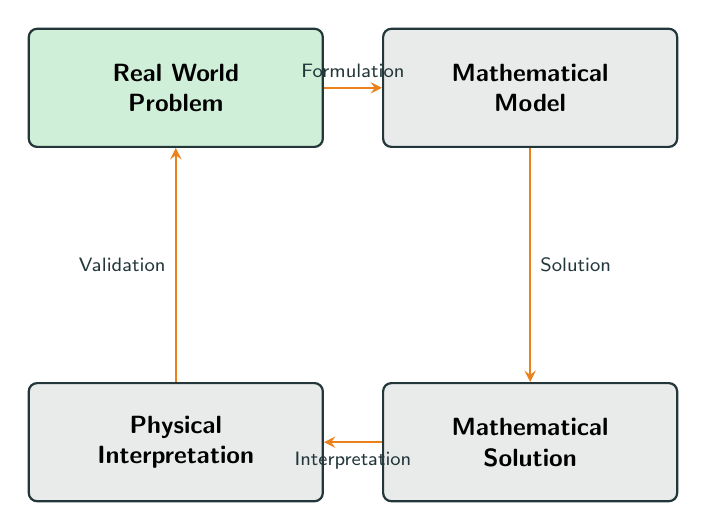
\begin{tikzpicture}[
            node distance=4.5cm, 
            auto,
            box/.style={
                draw, 
                rectangle, 
                rounded corners=3pt,
                text width=3.5cm, 
                text centered,
                minimum height=1.5cm,
                fill=mDarkTeal!10,
                draw=mDarkTeal,
                thick,
                font=\small\bfseries
            },
            arrow/.style={
                ->,
                thick,
                color=mLightBrown,
                >=stealth
            },
            label/.style={
                font=\scriptsize,
                color=mDarkTeal
            }
        ]
            \node (real) [box, fill=mLightGreen!20] {Real World\\Problem};
            \node (math) [box, right of=real] {Mathematical\\Model};
            \node (solution) [box, below of=math] {Mathematical\\Solution};
            \node (interpret) [box, left of=solution] {Physical\\Interpretation};
            
            \draw[arrow] (real) -- (math) node[midway, above, label] {Formulation};
            \draw[arrow] (math) -- (solution) node[midway, right, label] {Solution};
            \draw[arrow] (solution) -- (interpret) node[midway, below, label] {Interpretation};
            \draw[arrow] (interpret) -- (real) node[midway, left, label] {Validation};
        \end{tikzpicture}
    \end{center}
\end{frame}

\begin{frame}{Systematic Modeling Principles}
    \concept{Fundamental steps in rigorous mathematical modeling:}
    
    \vspace{0.3cm}
    
    \begin{enumerate}
        \item Identify the relevant variables and parameters within the system
        \item Formulate assumptions to simplify the complex real-world scenario
        \item Establish the governing differential equation(s)
        \item Solve the equation using analytical or numerical methods
        \item Interpret the mathematical solution in the physical context
        \item Validate the model against experimental or observational data
        \item Refine the model iteratively to improve accuracy
    \end{enumerate}
    
    \vspace{0.3cm}
    
    \emphasis{This systematic approach ensures robust and reliable mathematical representations of physical phenomena.}
\end{frame}

\begin{frame}{Case Study: Population Dynamics Model}
    \concept{Problem Statement:} Develop a mathematical model describing temporal population variations.
    
    \vspace{0.3cm}
    
    \concept{Fundamental Assumptions:}
    \begin{itemize}
        \item Birth rate exhibits proportionality to current population size
        \item Negligible mortality, immigration, and emigration effects
        \item Unlimited environmental resources and carrying capacity
    \end{itemize}
    
    \vspace{0.3cm}
    
    \concept{Mathematical Formulation:}
    \begin{equation}
        \frac{dP}{dt} = rP
    \end{equation}
    
    where $P(t)$ represents population at time $t$ and $r$ denotes the intrinsic growth rate parameter.
    
    \vspace{0.2cm}
    
    \emphasis{This fundamental model serves as the foundation for more sophisticated population dynamics theories.}
\end{frame}

\section{Curricular Structure and Academic Assessment}

\begin{frame}{Modular Curriculum Architecture}
    \concept{Thematic Module Organization:}
    
    \vspace{0.3cm}
    
    \begin{enumerate}
        \item First-Order Differential Equations (Sessions 2-4)
        \item Second-Order Differential Equations (Sessions 5-7)
        \item Power Series Solutions and Special Functions (Sessions 8-10)
        \item Laplace Transform Methods (Sessions 11-13)
        \item Non-Linear Differential Equations (Sessions 14-16)
        \item Partial Differential Equations (Sessions 17-19)
    \end{enumerate}
    
    \vspace{0.3cm}
    
    \concept{Culminating Session:} Comprehensive Review and Integrative Assessment (Session 20)
    
    \vspace{0.2cm}
    
    \emphasis{Each module builds systematically upon previous concepts, ensuring coherent knowledge development.}
\end{frame}

\begin{frame}{Comprehensive Assessment Framework}
    \concept{Evaluation Components and Weightings:}
    
    \vspace{0.3cm}
    
    \begin{itemize}
        \item 50\% Cumulative Theoretical-Practical Midterm Examinations
        \begin{itemize}
            \item[\textbullet] Administered after modules 2, 4, and 6 (sessions 7, 13, 19)
            \item[\textbullet] Emphasizes conceptual understanding and practical application
        \end{itemize}
        
        \item 20\% Activities, Assignments, and Integrating Cases
        \begin{itemize}
            \item[\textbullet] Conducted during practice sessions (4, 7, 10, 13, 16, 19)
            \item[\textbullet] Promotes active learning and skill development
        \end{itemize}
        
        \item 30\% Final Integrating Examination
        \begin{itemize}
            \item[\textbullet] Session 20 comprehensive assessment
            \item[\textbullet] Synthesizes knowledge across all course modules
        \end{itemize}
    \end{itemize}
\end{frame}

\begin{frame}{Academic Resources and Bibliography}
    \concept{Primary Textbook:}
    \begin{itemize}
        \item Nagle, R. Kent, et al. \textit{Fundamentals of Differential Equations and Boundary Value Problems}, 6th ed. Boston: Pearson Education, 2012.
    \end{itemize}
    
    \vspace{0.3cm}
    
    \concept{Supplementary Academic References:}
    \begin{itemize}
        \item Simmons, George F. \textit{Differential Equations with Applications and Historical Notes}, 2nd ed. New York: McGraw Hill, 1991.
        \item Boyce, W., DiPrima, R., Meade, D. \textit{Elementary Differential Equations and Boundary Value Problems}. Wiley, 2016.
        \item Zill, Dennis G. \textit{A First Course in Differential Equations with Modeling Applications}, 11th ed. Boston: Cengage Learning, 2017.
    \end{itemize}
    
    \vspace{0.2cm}
    
    \emphasis{These resources provide comprehensive theoretical foundations and practical applications essential for academic success.}
\end{frame}

\section{Course Progression and Preparation Guidelines}

\begin{frame}{Upcoming Academic Content}
    \concept{Next Session (Session 2):} First-Order Differential Equations - Theoretical Foundations
    
    \vspace{0.3cm}
    
    \concept{Topics for Examination:}
    \begin{itemize}
        \item Linear equations with variable coefficients
        \item Separable differential equations
        \item Advanced solution techniques and methodologies
        \item Initial value problems and boundary conditions
    \end{itemize}
    
    \vspace{0.3cm}
    
    \concept{Preparatory Requirements:}
    \begin{itemize}
        \item Comprehensive review of differential and integral calculus fundamentals
        \item Study Chapter 1 of the primary textbook (Nagle et al.)
        \item Practice advanced integration techniques and substitution methods
        \item Familiarize with mathematical notation and terminology
    \end{itemize}
\end{frame}

\begin{frame}{Academic Discourse and Inquiry}
    \begin{center}
        \Huge \concept{Questions and Academic Discussion}
        
        \vspace{1cm}
        
        \large Let us engage in scholarly discourse regarding the course structure, academic expectations, mathematical prerequisites, or any theoretical concepts requiring clarification.
        
        \vspace{0.5cm}
        
        \emphasis{Your active participation is essential for optimal learning outcomes.}
    \end{center}
\end{frame}

\begin{frame}[standout]
    \concept{Welcome to F1010!}\\
    \textbf{Modeling with Differential Equations}
    
    \vspace{1cm}
    
    \Large Are you prepared to embark upon this rigorous exploration of the mathematical foundations governing dynamic systems and temporal change?
    
    \vspace{0.5cm}
    
    \emphasis{Excellence in mathematical modeling awaits your dedication.}
\end{frame}

\end{document}
